%%%%%%%%%%%%%%%%%%%%%%%%%%%%%%%%%%%%%%%%%
% Arsclassica Article
% LaTeX Template
% Version 1.1 (10/6/14)
%
% This template has been downloaded from:
% http://www.LaTeXTemplates.com
%
% Original author:
% Lorenzo Pantieri (http://www.lorenzopantieri.net) with extensive modifications by:
% Vel (vel@latextemplates.com)
%
% License:
% CC BY-NC-SA 3.0 (http://creativecommons.org/licenses/by-nc-sa/3.0/)
%
%%%%%%%%%%%%%%%%%%%%%%%%%%%%%%%%%%%%%%%%%

%----------------------------------------------------------------------------------------
%	PACKAGES AND OTHER DOCUMENT CONFIGURATIONS
%----------------------------------------------------------------------------------------

\documentclass[
12pt, % Main document font size
a4paper, % Paper type, use 'letterpaper' for US Letter paper
oneside, % One page layout (no page indentation)
%twoside, % Two page layout (page indentation for binding and different headers)
headinclude,footinclude, % Extra spacing for the header and footer
BCOR5mm, % Binding correction
]{scrartcl}

%%%%%%%%%%%%%%%%%%%%%%%%%%%%%%%%%%%%%%%%%
% Arsclassica Article
% Structure Specification File
%
% This file has been downloaded from:
% http://www.LaTeXTemplates.com
%
% Original author:
% Lorenzo Pantieri (http://www.lorenzopantieri.net) with extensive modifications by:
% Vel (vel@latextemplates.com)
%
% License:
% CC BY-NC-SA 3.0 (http://creativecommons.org/licenses/by-nc-sa/3.0/)
%
%%%%%%%%%%%%%%%%%%%%%%%%%%%%%%%%%%%%%%%%%

%----------------------------------------------------------------------------------------
%	REQUIRED PACKAGES
%----------------------------------------------------------------------------------------

\usepackage[
nochapters, % Turn off chapters since this is an article        
beramono, % Use the Bera Mono font for monospaced text (\texttt)
eulermath,% Use the Euler font for mathematics
pdfspacing, % Makes use of pdftex’ letter spacing capabilities via the microtype package
dottedtoc % Dotted lines leading to the page numbers in the table of contents
]{classicthesis} % The layout is based on the Classic Thesis style

\usepackage{arsclassica} % Modifies the Classic Thesis package

\usepackage[T1]{fontenc} % Use 8-bit encoding that has 256 glyphs

\usepackage[utf8]{inputenc} % Required for including letters with accents

\usepackage{graphicx} % Required for including images
\graphicspath{{Figures/}} % Set the default folder for images

\usepackage{enumitem} % Required for manipulating the whitespace between and within lists

\usepackage{lipsum} % Used for inserting dummy 'Lorem ipsum' text into the template

\usepackage{subfig} % Required for creating figures with multiple parts (subfigures)

\usepackage{amsmath,amssymb,amsthm} % For including math equations, theorems, symbols, etc

\usepackage{varioref} % More descriptive referencing

\usepackage{tabularx} % http://tex.stackexchange.com/questions/15282/tabular-title-above-and-caption-below
\usepackage{ragged2e}
\usepackage{booktabs}
\usepackage{caption}

\usepackage{url} % http://stackoverflow.com/questions/2640111/url-latex-linebreak-problem

%----------------------------------------------------------------------------------------
%	THEOREM STYLES
%---------------------------------------------------------------------------------------

\theoremstyle{definition} % Define theorem styles here based on the definition style (used for definitions and examples)
\newtheorem{definition}{Definition}

\theoremstyle{plain} % Define theorem styles here based on the plain style (used for theorems, lemmas, propositions)
\newtheorem{theorem}{Theorem}

\theoremstyle{remark} % Define theorem styles here based on the remark style (used for remarks and notes)

%----------------------------------------------------------------------------------------
%	HYPERLINKS
%---------------------------------------------------------------------------------------

\hypersetup{
%draft, % Uncomment to remove all links (useful for printing in black and white)
colorlinks=true, breaklinks=true, bookmarks=true,bookmarksnumbered,
urlcolor=webbrown, linkcolor=RoyalBlue, citecolor=webgreen, % Link colors
pdftitle={}, % PDF title
pdfauthor={\textcopyright}, % PDF Author
pdfsubject={}, % PDF Subject
pdfkeywords={}, % PDF Keywords
pdfcreator={pdfLaTeX}, % PDF Creator
pdfproducer={LaTeX with hyperref and ClassicThesis} % PDF producer
} % Include the structure.tex file which specified the document structure and layout

\hyphenation{Fortran hy-phen-ation} % Specify custom hyphenation points in words with dashes where you would like hyphenation to occur, or alternatively, don't put any dashes in a word to stop hyphenation altogether

%----------------------------------------------------------------------------------------
%	TITLE AND AUTHOR(S)
%----------------------------------------------------------------------------------------

\title{\normalfont\spacedallcaps{Whitehouse.gov usability report}} % The article title

\author{\spacedlowsmallcaps{Enrico Rotundo*, 1008052}} % The article author(s) - author affiliations need to be specified in the AUTHOR AFFILIATIONS block

\date{August, 2014} % An optional date to appear under the author(s)

%----------------------------------------------------------------------------------------

\begin{document}

%----------------------------------------------------------------------------------------
%	HEADERS
%----------------------------------------------------------------------------------------

\renewcommand{\sectionmark}[1]{\markright{\spacedlowsmallcaps{#1}}} % The header for all pages (oneside) or for even pages (twoside)
%\renewcommand{\subsectionmark}[1]{\markright{\thesubsection~#1}} % Uncomment when using the twoside option - this modifies the header on odd pages
\lehead{\mbox{\llap{\small\thepage\kern1em\color{halfgray} \vline}\color{halfgray}\hspace{0.5em}\rightmark\hfil}} % The header style

\pagestyle{scrheadings} % Enable the headers specified in this block


%----------------------------
% CUSTOM COMMAND
%----------------------------

\newcommand{\thesite}{\href{http://www.whitehouse.gov/}{whitehouse.gov}}

%----------------------------------------------------------------------------------------
%	TABLE OF CONTENTS & LISTS OF FIGURES AND TABLES
%----------------------------------------------------------------------------------------

\maketitle % Print the title/author/date block

\setcounter{tocdepth}{2} % Set the depth of the table of contents to show sections and subsections only

\tableofcontents % Print the table of contents

\listoffigures % Print the list of figures

% \listoftables % Print the list of tables

%----------------------------------------------------------------------------------------
%	ABSTRACT
%----------------------------------------------------------------------------------------

%\section*{Abstract} % This section will not appear in the table of contents due to the star (\section*)

%\lipsum[1] % Dummy text

%----------------------------------------------------------------------------------------
%	AUTHOR AFFILIATIONS
%----------------------------------------------------------------------------------------

{\let\thefootnote\relax\footnotetext{* \textit{Computer Science BSc student, Department of Mathematics, Univerisity of Padua, Italy}}}

%----------------------------------------------------------------------------------------

\newpage % Start the article content on the second page, remove this if you have a longer abstract that goes onto the second page

%----------------------------------------------------------------------------------------
%	INTRODUCTION
%----------------------------------------------------------------------------------------

\section{Introduction}
	This documents is a usability report of the website \thesite{}, following referred as ``the site'' or ``the webiste''. The website analized represent the US government, it's focused on the person of the President and deliver high grained informations about him and Administration activities.  
 
%----------------------------------------------------------------------------------------
%	NAME AND DOMAIN
%----------------------------------------------------------------------------------------

\section{Name and domain}

The website name is the same of the institutions that represent, its meaning is unambiguous all around the world, so it's enough well-known to be clear and immediate. The domain is \emph{.gov} that clearly represent an official government website so its choice is appropriate. Others domains, like \emph{.com}/\emph{.org}/\emph{.it}, doesen't redirect to \thesite{} and seems to be not related to the government. Since the website is a sensible target, i would expect that at least the \emph{.com} redirects to the main one, simply to avoid possible attacks like website cloning.

%----------------------------------------------------------------------------------------
%	HOMEPAGE
%----------------------------------------------------------------------------------------

\newpage
\section{Homepage}

\begin{figure}[h]
\centering 
\centerline{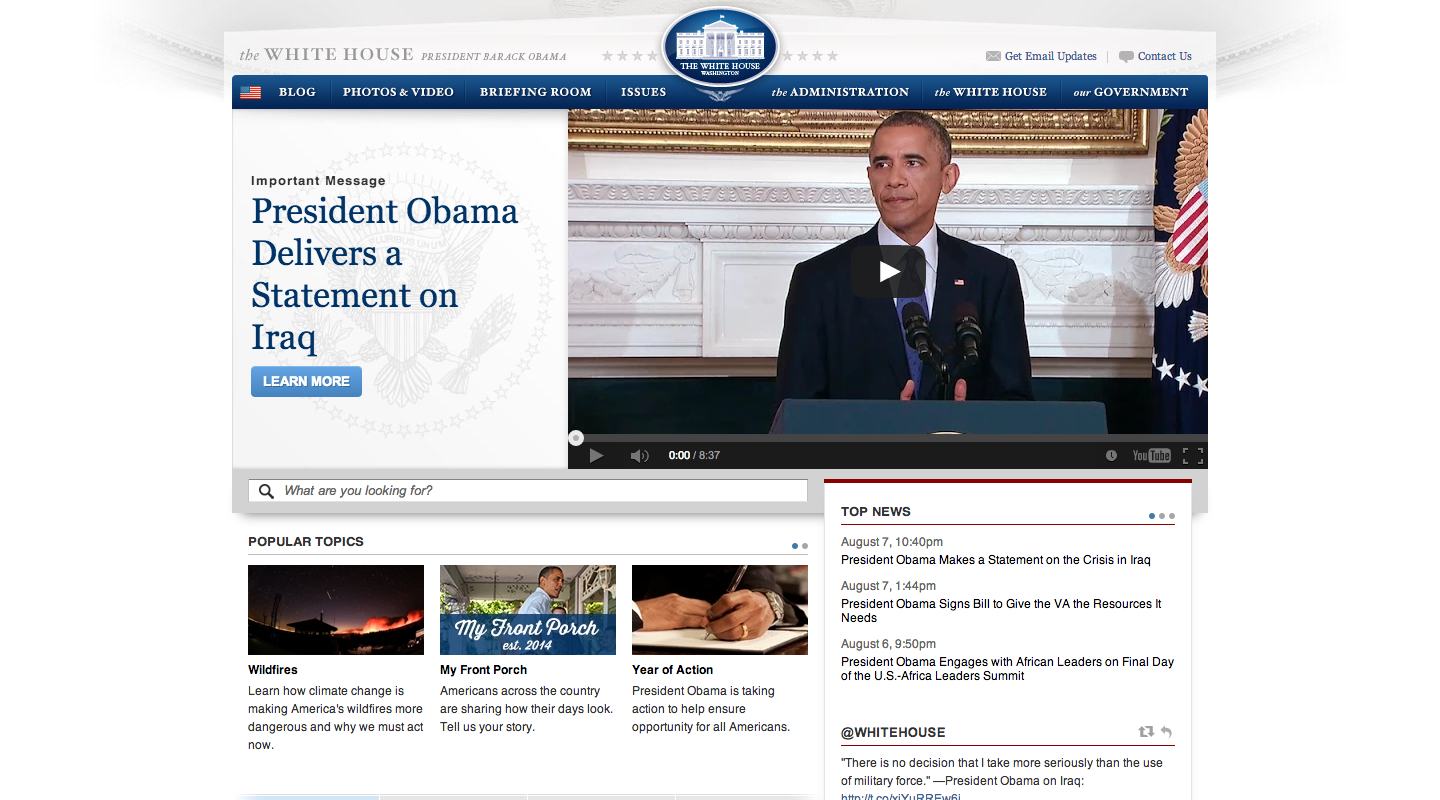
\includegraphics[width=1.8\columnwidth]{homepage-visible}}
\caption[Homepage]{Homepage of \thesite{}}
\label{fig:homepage} 
\end{figure}

The 6w's\footnote{included ``How'', \url{http://en.wikipedia.org/wiki/Five_Ws}} axis ..... %TODO

\begin{itemize}[noitemsep]
	\item \textit{Where:} where are we? The subtitle isn't that decriptive but the words \emph{whitehouse} and \emph{President Barack Obama} together clearify where we are. The breadcrumb lack doesn't explain where we are positioned inside the website, this fact could create user disorientation.

	\item \textit{Who:}


	\item \textit{Why:}
	\item \textit{What:} 
	\item \textit{When:}
	\item \textit{How:}
\end{itemize}

%----------------------------------------------------------------------------------------
%	INTERNAL PAGES
%----------------------------------------------------------------------------------------

\section{Internal pages}
	
	\subsection{pag1}

	\subsection{pag2}

	\subsection{pag3}


%----------------------------------------------------------------------------------------
%	GENERALS OBSERVATIONS
%----------------------------------------------------------------------------------------

\section{General observations}


%----------------------------------------------------------------------------------------
%	SUMMARY
%----------------------------------------------------------------------------------------

\section{SUMMARY}


%----------------------------------------------------------------------------------------
%	LIST OF FIGURES
%----------------------------------------------------------------------------------------

\section{List of figures}

% %----------------------------------------------------------------------------------------
% %	
% %----------------------------------------------------------------------------------------

% \section{}



%----------------------------------------------------------------------------------------
%	BIBLIOGRAPHY
%----------------------------------------------------------------------------------------

% \renewcommand{\refname}{\spacedlowsmallcaps{References}} % For modifying the bibliography heading

% \bibliographystyle{unsrt}

% \bibliography{sample.bib} % The file containing the bibliography

%----------------------------------------------------------------------------------------

\end{document}